\chapter{\texorpdfstring{\(SU(5)\)}{5} 다중항, 렙토쿼크 게이지 보손과 양성자 붕괴}

\lectureoverview{표준 모형의 군을 \(SU(5)\)에 포함하면 대통일이 구체적인 형태를 갖는다. 이 말의 뜻을 이해하기 위해 먼저 필요한 표현론을 살펴보자. 기본 표현 \(N\)과 그 켤레 표현 \(\overline N\), 텐서곱, 대칭 및 반대칭 텐서, 그리고 수반 표현이 그것이다. 그러면 표준 모형의 한 세대가 놀라울 만큼 간결한 조합 \(\overline{\mathbf 5}\oplus\mathbf{10}\)으로 묶인다. 이 구성을 아름답게 만드는 대칭성은 쿼크를 렙톤으로 바꾸는 색전하 게이지 보손도 요구한다. 이 보손의 교환은 양성자 붕괴를 허용하므로 통일 에너지 척도는 \(10^{15}\)--\(10^{16}\,\mathrm{GeV}\) 부근이어야 한다. 게이지 결합상수의 에너지에 따른 변화도 비슷한 척도를 가리킨다. 마지막에 초대칭을 다시 살펴보는 이유는 초대칭을 포함하면 결합상수들이 만나는 값이 수치상 훨씬 더 정확하게 일치하기 때문이다.}

\section{군 표현부터 시작하는 이유}

대통일 이론은 여러 가지가 제안되어 있다. 이론들을 두루 살펴보는 대신, 한 가지 사례를 뜯어보며 세 가지를 묻겠다. 무엇이 이 이론을 성립하게 하는가? 어떤 새 입자들이 필요한가? 실험은 이 이론을 어디에서 위태롭게 하는가? 여기서 다룰 군은 \(SU(5)\)이며, 그 구조의 핵심은 다음 포함 관계다.
\begin{equation}
SU(3)_c\times SU(2)_L\times U(1)_Y
\subset SU(5).
\label{eq:l10-sm-embedding}
\end{equation}
여기서 \(SU(3)_c\)은 색에, \(SU(2)_L\)은 약한 아이소스핀에, \(U(1)_Y\)은 약한 하이퍼전하에 작용한다.

초대칭은 이 구성의 전제가 아니다. 초대칭이 대통일을 논리적으로 함의하지도 않고, 대통일이 초대칭을 함의하지도 않는다. 이 강의에서 둘의 연결고리는 수치적이다. 초짝입자 스펙트럼을 재규격화군 계산에 포함하면 세 게이지 결합상수가 공통값에 더 정확하게 가까워진다.

대칭 변환이 서로 섞는 입자들은 대칭군의 표현을 이룬다. 따라서 통일된 입자 다중항을 분류하려면 먼저 표현론을 조금 살펴볼 필요가 있다.

\subsection{익숙한 \texorpdfstring{\(SU(2)\)}{2} 예}

보통 각운동량과 관련된 \(SU(2)\)은 3차원 공간의 회전과 밀접하게 연관되어 있다. 더 정확히 말하면, \(SU(2)\)은 \(SO(3)\)의 이중 덮개다. 그 기약 표현은 다음과 같이 표기한다.
\begin{equation}
j=0,\frac12,1,\frac32,\ldots,
\qquad
\dim(j)=2j+1.
\label{eq:l10-su2-spins}
\end{equation}
따라서 스칼라는 단일항이고, 스핀 \(\tfrac12\) 입자는 이중항이며, 스핀 1 입자는 삼중항이다. 약한 상호작용의 군 \(SU(2)_L\)은 물리적으로는 다른 대칭이지만, 추상적인 군론은 같다.

\section{기본 표현과 그 켤레 표현}

\(SU(N)\)에서 기본 표현은 복소수 \(N\)성분 열벡터들의 공간이다.
\begin{equation}
\psi=
\begin{pmatrix}
\psi_1\\
\psi_2\\
\vdots\\
\psi_N
\end{pmatrix},
\qquad
\psi'_i=U_i{}^j\psi_j,
\qquad
U\in SU(N).
\label{eq:l10-defining}
\end{equation}
이를 기본 표현이라고 하거나 간단히 \(\mathbf N\)라고 부른다. 행렬 \(U\)은 \(N\times N\) 행렬이며, 이 행렬이 작용하는 벡터 공간의 차원은 \(N\)이다.

복소켤레를 취하면 또 하나의 \(N\)차원 표현을 얻는다.
\begin{equation}
\psi_i^*\longmapsto U_i{}^{j*}\psi_j^*,
\label{eq:l10-conjugate}
\end{equation}
이를 \(\overline{\mathbf N}\)로 표기한다. \(N>2\)에서는 기본 표현과 켤레 표현이 동등하지 않다. 어느 쪽을 입자 표현으로, 어느 쪽을 반입자 표현으로 부를지는 바꿀 수 있지만, 관례를 정한 뒤에는 일관되게 유지해야 한다.

\begin{classroomqa}\audiencequestion{\(N\)가 \(SU(N)\)에서 \(N\)이 짝수인지 홀수인지에 따라 달라지나요? 행렬을 가리키는 건가요? \lecturetimestamp{00:07:33}}
\lecturerresponse{여기에는 짝수--홀수에 따른 제한이 없습니다. \(N\)은 기본 행렬의 크기이자 기본 표현의 차원이기도 합니다. \(\mathbf N\)와 \(\overline{\mathbf N}\)은 둘 다 그 차원을 갖습니다.}
\end{classroomqa}

반입자의 반입자는 원래 입자다. 그러므로 \(\mathbf N\)와 \(\overline{\mathbf N}\)의 이름을 서로 바꾸는 것은 물리학이 아니라 관례를 바꾸는 일이다.

\section{텐서곱과 기약성}

한 물체가 \(N\)개의 내부 상태를 가질 수 있고, 다른 물체도 독립적으로 똑같은 수의 상태를 가질 수 있다고 하자. 위치, 운동량, 스핀 및 이 \(SU(N)\) 표지 외의 모든 양자수를 무시하면 두 물체의 쌍은
\begin{equation}
N\times N=N^2
\label{eq:l10-product-count}
\end{equation}
개의 상태를 갖는다. 첫 번째 물체가 상태 \(\psi_i\)에 있고 두 번째 물체가 상태 \(\phi_j\)에 있다면, 그 곱은 다음과 같이 쓸 수 있다.
\begin{equation}
\Psi_{ij}=\psi_i\phi_j,
\qquad
\Psi'_{ij}=U_i{}^kU_j{}^\ell\Psi_{k\ell}.
\label{eq:l10-tensor-transform}
\end{equation}
이것이 텐서곱 \(\mathbf N\otimes\mathbf N\)이다.

\begin{classroomqa}\audiencequestion{왜 답이 \(N^2\)인가요? \(N^2-1\)이 아닌가요? 두 입자가 같은 내부 표지를 갖도록 허용하면 배타 원리를 위반하지 않나요? \lecturetimestamp{00:10:22}}
\lecturerresponse{여기서는 두 자리가 구별된다. 한 물체는 한 위치에 고정되어 있고 다른 물체는 다른 위치에 있다. 파울리 원리는 위치를 포함한 완전한 양자 상태에 제약을 가한다. 이 원리가 \(N^2\)개의 내부 표지 조합을 제거하지는 않는다. \(N^2-1\)이라는 수는 뒤에서 다른 곱에 무흔적 조건을 적용할 때 나온다.}
\end{classroomqa}

차원 \(N^2\)인 곱 표현은 일반적으로 가약이다. 표현에 군의 작용을 받아도 그 안에 머무는 진부분공간이 있으면 그 표현을 가약이라 한다. 이런 불변 부분공간을 분리해 더 작은 표현으로 다룰 수 있다. 그러한 진부분공간이 하나도 없으면 그 표현은 기약이다.

\subsection{대칭 텐서와 반대칭 텐서}

모든 2계 텐서는 다음 두 부분으로 유일하게 분해된다.
\begin{align}
\Psi_{ij}
&=\Psi^{(S)}_{ij}+\Psi^{(A)}_{ij},\\
\Psi^{(S)}_{ij}
&=\frac12(\Psi_{ij}+\Psi_{ji}),\\
\Psi^{(A)}_{ij}
&=\frac12(\Psi_{ij}-\Psi_{ji}).
\label{eq:l10-sym-anti}
\end{align}
두 부분은 다음 성질을 만족한다.
\begin{equation}
\Psi^{(S)}_{ij}=\Psi^{(S)}_{ji},
\qquad
\Psi^{(A)}_{ij}=-\Psi^{(A)}_{ji}.
\end{equation}
식~\eqref{eq:l10-tensor-transform}은 각각의 조건을 보존하므로 군 변환으로 대칭 부문과 반대칭 부문이 서로 섞이지 않는다.

\editorialnote{강의에서는 일반적인 경우의 셈을 연습문제로 남겨 두었다. 대칭 및 반대칭 부분공간의 차원은 각각 \(N(N+1)/2\)와 \(N(N-1)/2\)이며, 두 차원을 더하면 \(N^2\)이다.}

\begin{figure}[htbp]\centering
\includegraphics[width=0.78\textwidth]{lecture_10_figure_02.png}\lectureframe{00:17:57.500}\caption{스핀 \(\tfrac12\) 상태 두 개를 대칭 상태 세 개와 반대칭 상태 하나로 완전히 분해한 판서.}\label{fig:l10-spin-decomposition}\end{figure}

\(SU(2)\)의 기본 이중항에 대해,
\begin{equation}
\mathbf2\otimes\mathbf2=\mathbf3_S\oplus\mathbf1_A.
\label{eq:l10-two-two}
\end{equation}
두 기저 상태를 \(u\)와 \(d\)로 쓰면, 대칭 삼중항은 다음과 같다.
\begin{align}
\ket{1,1}&=\ket{uu},\\
\ket{1,0}&=\frac{1}{\sqrt2}\bigl(\ket{ud}+\ket{du}\bigr),\\
\ket{1,-1}&=\ket{dd},
\end{align}
반면 반대칭 단일항은 다음과 같다.
\begin{equation}
\ket{0,0}
=\frac{1}{\sqrt2}\bigl(\ket{ud}-\ket{du}\bigr).
\end{equation}
이것은 스핀 \(\tfrac12\) 각운동량 두 개를 더하는 익숙한 결과다. 원래의 네 상태가 스핀 1과 스핀 0으로 재구성된다.

\section{입자와 반입자: 수반 표현}

이제 기본 표현과 그 켤레 표현을 결합하자. 곱에는 여전히 \(N^2\)개의 성분이 있지만, 행렬처럼 변환한다.
\begin{equation}
M_i{}^j\in\mathbf N\otimes\overline{\mathbf N},
\qquad
M\longmapsto U M U^\dagger.
\label{eq:l10-matrix-transform}
\end{equation}
\(\mathbf N\otimes\mathbf N\)과 달리 기본 표현 지표 하나와 반기본 표현 지표 하나 사이에는 의미 있는 교환 대칭이 없다. 대신 자연스러운 분해는 다음과 같다.
\begin{equation}
M
=
\frac{\operatorname{tr}M}{N}\,\mathbf1_N
+
\left(M-\frac{\operatorname{tr}M}{N}\,\mathbf1_N\right).
\label{eq:l10-trace-split}
\end{equation}
첫 번째 항은 단일항이고, 무흔적 부분은 수반 표현이다.
\begin{equation}
\mathbf N\otimes\overline{\mathbf N}
=\mathbf1\oplus\mathbf{Adj},
\qquad
\dim\mathbf{Adj}=N^2-1.
\label{eq:l10-adjoint}
\end{equation}

\begin{figure}[htbp]\centering
\includegraphics[width=0.67\textwidth]{lecture_10_figure_04.png}\lectureframe{00:23:47.500}\caption{\(\mathbf N\otimes\overline{\mathbf N}\)의 무흔적 성분 \(N^2-1\)개가 수반 표현을 이룬다는 판서의 결론.}\label{fig:l10-adjoint}\end{figure}

\(SU(3)\)에서는 익숙한 팔중항을 얻는다.
\begin{equation}
\mathbf3\otimes\overline{\mathbf3}
=\mathbf8\oplus\mathbf1,
\end{equation}
8개의 글루온은 수반 표현으로 변환한다. \(SU(2)\)에서는 수반 표현의 차원이 3이며 스핀 1처럼 변환한다.

\section{표준 모형의 한 세대}

관측된 세대는 세 개지만, \(SU(5)\)은 각 세대에 같은 구성을 별도로 적용한다. 세 복사본이 존재하는 이유까지 설명하지는 않는다. 따라서 첫 번째 세대에 초점을 맞추자.

모든 장은 왼손잡이 바일 장으로 쓰겠다. 오른손잡이 페르미온은 왼손잡이 전하켤레 장으로 나타낸다.
\begin{equation}
u^c_L,\qquad d^c_L,\qquad e^c_L.
\label{eq:l10-left-handed-bookkeeping}
\end{equation}
위첨자 \(c\)은 전하켤레를 뜻한다. 예를 들어 \(d^c_L\)은 전기 전하가 \(+\tfrac13\)인 왼손잡이 반다운 쿼크 장이다.

표준적인 \(SU(5)\) 표기법에서 왼손잡이 장 15개 중 다섯 개는 다음 표현에 들어간다.
\begin{equation}
\overline{\mathbf5}
=
\begin{pmatrix}
\nu_{eL}\\
e_L\\
d^c_{rL}\\
d^c_{gL}\\
d^c_{bL}
\end{pmatrix}.
\label{eq:l10-fivebar}
\end{equation}
약한 상호작용의 2차원 블록을 먼저 쓰고 색의 3차원 블록을 뒤에 쓰도록 순서를 정했다. 약한 상호작용의 변환은 앞의 두 성분을 서로 섞고, 색 변환은 마지막 세 성분을 서로 섞는다. 비대각 \(SU(5)\) 생성자는 두 블록을 연결한다.

\editorialnote{강의에서는 식~\eqref{eq:l10-fivebar}의 열벡터를 \(\mathbf5\)라고 부르고, 뒤에서는 반대칭 다중항을 \(\overline{\mathbf{10}}\)라고 부른다. 이는 모든 표현을 전역적으로 켤레화한 관례다. 여기서는 현대 표준 관례 \(\overline{\mathbf5}\oplus\mathbf{10}\)를 사용한다. 모든 표현을 켤레화하면 물리학은 그대로 둔 채 강의의 명칭을 재현할 수 있다.}

최소 모형에서 첫 세대의 전체 구성은 다음과 같다.
\begin{equation}
\begin{gathered}
\underbrace{Q_L=(u_L,d_L)}_{6}
\oplus
\underbrace{L_L=(\nu_{eL},e_L)}_{2},\\
\underbrace{u^c_L}_{3}
\oplus
\underbrace{d^c_L}_{3}
\oplus
\underbrace{e^c_L}_{1},\\
6+2+3+3+1=15.
\end{gathered}
\label{eq:l10-fifteen}
\end{equation}
최소 표준 모형에는 독립적인 \(\nu^c_L\)가 없으므로 재규격화 가능한 중성미자 질량을 줄 수 없다. 중성미자 진동은 이 최소 모형의 설명이 불완전함을 보여 준다. 자연에는 영이 아닌 작은 중성미자 질량이 있으며, 이를 설명하려면 모형을 확장해야 한다.

\begin{classroomqa}\audiencequestion{페르미온 질량이 왼손잡이 상태를 오른손잡이 상태로 바꿀 때, 입자도 반입자로 바뀌나요? \lecturetimestamp{00:34:00}}
\lecturerresponse{아니다. 전자 질량은 왼손잡이 전자와 전기 전하가 같은 오른손잡이 전자를 연결한다. 모든 장을 왼손잡이로 쓰는 표기법에서는 두 번째 장을 \(e^c_L\)로 나타내지만, 4성분 입자는 여전히 전자다. 입자와 반입자를 동일시하는 마요라나 질량을 가질 수 있는 것은 중성 장뿐이다.}
\end{classroomqa}

\section{다중항에서 드러나는 게이지 보손}

게이지 대칭의 각 생성자에는 그에 대응하는 게이지 장이 있다. 식~\eqref{eq:l10-fivebar}에는 익숙한 전이들이 이미 드러나 있다.
\begin{itemize}
\item 약한 게이지 장은 \(\nu_{eL}\)와 \(e_L\) 사이에서 작용한다.
\item 글루온은 \(d^c_L\)의 세 색 사이에서 작용한다.
\item 중성 생성자는 대각 성분으로 작용한다.
\item 새로운 비대각 생성자는 렙톤 성분과 색을 띤 성분을 서로 바꾼다.
\end{itemize}

글루온이 쿼크--반쿼크 색 양자수를 지닌다고 그려 볼 수 있다. 강의에서는 통상적인 세계선 기억법을 사용한다. 방출 정점을 지나 나가는 반쿼크를 거꾸로 따라가면 앞으로 움직이는 쿼크처럼 보인다. 따라서 방출된 장은 쿼크--반쿼크 쌍의 양자수를 지닌다. 표현론의 언어로는 이것이 정확히 \(\mathbf3\otimes\overline{\mathbf3}\)의 무흔적 부분이다.

\(SU(5)\)에서,
\begin{equation}
\dim\mathbf{Adj}_{SU(5)}=5^2-1=24.
\end{equation}
표준 모형 부분군 아래에서 이 게이지 장들은 다음과 같이 분해된다.
\begin{equation}
\mathbf{24}
=
(\mathbf8,\mathbf1)_0
\oplus(\mathbf1,\mathbf3)_0
\oplus(\mathbf1,\mathbf1)_0
\oplus(\mathbf3,\mathbf2)_{-5/6}
\oplus(\overline{\mathbf3},\mathbf2)_{5/6},
\label{eq:l10-adjoint-sm}
\end{equation}
여기서 순서쌍은 \(SU(3)_c\times SU(2)_L\)을 나타내며, 아래 첨자는 하이퍼전하다.

\editorialnote{식~\eqref{eq:l10-adjoint-sm}은 강의에서 그린 블록 구조를 명확히 보여 준다. 처음 세 항에는 익숙한 색 및 전약 게이지 장이 들어 있다. 마지막 두 항은 관례적으로 \(X\) 보손과 \(Y\) 보손이라 부르는 실수 자유도 12개를 나타낸다.}

\begin{figure}[htbp]\centering
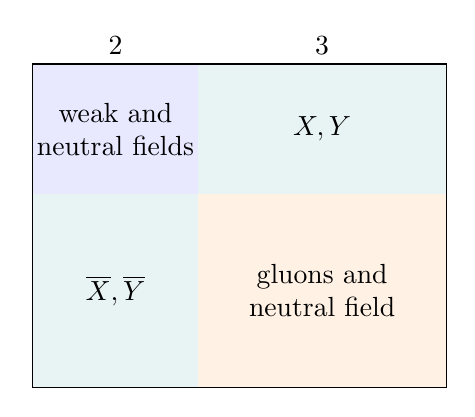
\begin{tikzpicture}[x=1.05cm,y=0.82cm]
  \draw[thick] (0,0) rectangle (5,5);
  \draw[thick] (2,0) -- (2,5);
  \draw[thick] (0,3) -- (5,3);
  \fill[blue!9] (0,3) rectangle (2,5);
  \fill[orange!10] (2,0) rectangle (5,3);
  \fill[teal!9] (2,3) rectangle (5,5);
  \fill[teal!9] (0,0) rectangle (2,3);
  \node[align=center] at (1,4) {weak and\\neutral fields};
  \node[align=center] at (3.5,1.5) {gluons and\\neutral field};
  \node[align=center] at (3.5,4) {\(X,Y\)};
  \node[align=center] at (1,1.5) {\(\overline X,\overline Y\)};
  \node[above] at (1,5) {\(2\)};
  \node[above] at (3.5,5) {\(3\)};
\end{tikzpicture}\caption{\(2\oplus3\) 구조를 가진 \(SU(5)\) 게이지 장. 비대각 블록이 렙톤과 색을 띤 장을 연결한다.}\label{fig:l10-gauge-blocks}\end{figure}

\(Q=T_3+Y\)일 때, 식~\eqref{eq:l10-adjoint-sm}의 색을 띤 약한 이중항은 전하 \(-\tfrac13\)와 \(-\tfrac43\)를 갖고, 그 켤레는 \(+\tfrac13\)와 \(+\tfrac43\)를 갖는다. 강의에서는 이 입자들을 \(X\)와 \(Y\)라고 부르지만, 어느 이름이 어느 전하에 해당하는지는 명시적으로 정하지 않는다. 전이와 전하가 관례와 무관한 내용이다.

\begin{classroomqa}\audiencequestion{새로운 \(X\) 보손 또는 \(Y\) 게이지 보손은 각각 세 종류인가요? \lecturetimestamp{00:41:28}}
\lecturerresponse{그렇다. 전이는 색을 띤 쿼크 성분과 색이 없는 렙톤 성분을 연결하므로, 교환되는 보손은 그 사이의 색 차이를 지녀야 한다. \(X/Y\) 장은 색 삼중항을 이루며 글루온을 방출하거나 흡수할 수 있다.}
\end{classroomqa}

색을 띤 입자는 고립된 점근 상태로 관측되지 않는다. 쿼크와 마찬가지로 새 게이지 보손도 붕괴하거나 강입자화하여 색중성 조합을 이루어야 한다.

\section{다중항에 반다운 쿼크가 들어가는 이유}

\(SU(N)\)의 생성자는 무흔적 에르미트 행렬이다. ‘특수’라는 말과의 연관을 보려면 무한소 군 원소를 다음과 같이 쓰면 된다.
\begin{equation}
U(\epsilon)=e^{i\epsilon T}.
\end{equation}
유니터리성으로부터 \(T^\dagger=T\)을 얻고,
\begin{equation}
1=\det U=e^{i\epsilon\operatorname{tr}T}
\end{equation}
임의의 \(\epsilon\)에 대해 다음이 성립하므로,
\begin{equation}
\operatorname{tr}T=0.
\label{eq:l10-traceless-generator}
\end{equation}

전기 전하는 생성자들의 선형 결합이다. 식~\eqref{eq:l10-fivebar}의 물질 열벡터에 작용할 때는 다음과 같다.
\begin{equation}
Q_{\overline5}
=
\operatorname{diag}
\left(0,-1,\frac13,\frac13,\frac13\right),
\qquad
\operatorname{tr}Q_{\overline5}=0.
\label{eq:l10-charge-fivebar}
\end{equation}
따라서
\begin{equation}
0-1+3\left(\frac13\right)=0.
\end{equation}
반다운 장을 다운 장으로 바꾸면 다음을 얻게 된다.
\begin{equation}
0-1+3\left(-\frac13\right)=-2,
\end{equation}
이 값은 \(SU(5)\) 생성자의 대각합일 수 없다. 그러므로 얼핏 이상해 보이는 반다운 배정은 군의 구조가 강제한다.

\section{나머지 페르미온 열 개}

나머지 장 열 개는 반대칭 2계 텐서에서 나온다. 표준 관례에서는 다음 표현의 반대칭 부분이다.
\begin{equation}
\mathbf5\otimes\mathbf5
=\mathbf{15}_S\oplus\mathbf{10}_A.
\label{eq:l10-five-five}
\end{equation}
강의에서는 잠시 켤레 양자수를 다음과 같이 써서 이 텐서를 구성한다.
\begin{equation}
\chi=
\begin{pmatrix}
\nu^c\\
e^c\\
d_r\\
d_g\\
d_b
\end{pmatrix}.
\label{eq:l10-aux-five}
\end{equation}
이는 표현의 텐서곱을 다루기 위한 계산상의 편의일 뿐, 합성 입자로 이루어진 물리적 5중항이 하나 더 존재한다는 뜻은 아니다.

다음과 같이 두자.
\begin{equation}
\Psi^{ij}=-\Psi^{ji},
\qquad
i,j=1,\ldots,5.
\label{eq:l10-antisym-ten}
\end{equation}
모든 대각 성분은 사라지고, 아래쪽 삼각 부분은 위쪽 삼각 부분으로 정해진다. 따라서
\begin{equation}
\dim\mathbf{10}
=\binom52
=\frac{5\cdot4}{2}
=10.
\label{eq:l10-ten-count}
\end{equation}

식~\eqref{eq:l10-aux-five}에서 각 성분의 전하는 해당 행과 열의 전하를 더한 값이다. 이에 따라 약한--약한 블록에는 \(e^c\)가 들어가고, 약한--색 블록에는 다운 및 업 쿼크가, 색--색 블록에는 반업 장이 들어간다.

\begin{classroomqa}\audiencequestion{양전자와 다운 쿼크의 표지를 결합하면 그 성분은 \(X\) 보손이어야 하나요? \lecturetimestamp{00:53:08}}
\lecturerresponse{아니다. 여기서는 게이지 보손 수반 표현이 아니라 페르미온 표현을 구성하고 있다. 전하를 더하면 \(1-\tfrac13=\tfrac23\)이므로 그 성분은 업 쿼크의 양자수를 갖는다.}
\end{classroomqa}

색에 일관된 부호를 택하면 다음과 같다.
\begin{equation}
\Psi^{ij}=
\begin{pmatrix}
0 & e^c & d_r & d_g & d_b\\
-e^c & 0 & u_r & u_g & u_b\\
-d_r & -u_r & 0 & u_b^c & -u_g^c\\
-d_g & -u_g & -u_b^c & 0 & u_r^c\\
-d_b & -u_b & u_g^c & -u_r^c & 0
\end{pmatrix}.
\label{eq:l10-ten-matrix}
\end{equation}
장 위상을 바꾸면 식에 표시된 부호 일부는 달라지지만, 표현과 입자 내용은 변하지 않는다.

\begin{figure}[htbp]\centering
\includegraphics[width=0.83\textwidth]{lecture_10_figure_05.png}\lectureframe{00:59:17.500}\caption{\(2\oplus3\) 성분과 색 표지를 확인한 뒤, 가림 없이 완성한 반대칭 물질 행렬.}\label{fig:l10-ten-board}\end{figure}

\begin{classroomqa}\audiencequestion{10차원 표현은 반드시 행렬로 써야 하나요? 열벡터로 쓸 수도 있나요? \lecturetimestamp{00:56:24}}
\lecturerresponse{둘 다 가능하다. 서로 독립인 성분 열 개를 열벡터에 나열할 수도 있다. 하지만 반대칭 \(5\times5\) 행렬은 \(SU(5)\)이 두 지표에 어떻게 작용하는지 보여 주므로 정보가 훨씬 많다.}
\end{classroomqa}

\begin{classroomqa}\audiencequestion{색--색 블록에서 \(u\)로 표시된 성분은 실제로 반업 장이어야 하지 않나요? \lecturetimestamp{00:57:51}}
\lecturerresponse{그렇다. 판서의 표지를 \(u^c\)로 고친다. 이는 왼손잡이 반업 장이다. 다운형 두 기저 전하를 더하면 \(-\tfrac23\)이 되며, 이는 반업 쿼크의 전기 전하다.}
\end{classroomqa}

\begin{classroomqa}\audiencequestion{행렬의 여러 성분에서 색 표지가 빠져 있습니다. 그래도 색은 보존되나요? \lecturetimestamp{00:58:05}}
\lecturerresponse{그렇다. 세 색 성분은 빨강, 초록, 파랑이다. 표지는 판서를 간결하게 하려고 생략했을 뿐이다.}
\end{classroomqa}

색 기본 표현 두 개의 반대칭 쌍은 반색으로 변환한다.
\begin{equation}
\wedge^2\mathbf3\simeq\overline{\mathbf3},
\qquad
(rg,rb,gb)\sim(\overline b,-\overline g,\overline r).
\label{eq:l10-anticolor}
\end{equation}
따라서 색--색 블록의 서로 다른 세 성분은 정확히 반업 색 삼중항을 이룬다.

이제 한 세대를 다음과 같이 구성했다.
\begin{equation}
\overline{\mathbf5}\oplus\mathbf{10}.
\label{eq:l10-family}
\end{equation}
\(u_L\)와 \(u^c_L\)가 하나의 기약 다중항 안에 함께 들어가지만, \(d_L\)와 \(d^c_L\), 그리고 \(e_L\)와 \(e^c_L\)는 서로 다른 다중항에 속한다는 점이 눈에 띈다.

\begin{classroomqa}\audiencequestion{게이지 변환이 각 표현 안에서만 작용한다면, 오중항막대와 십중항에 속한 장들을 질량 항이 어떻게 연결할 수 있나요? \lecturetimestamp{01:00:40}}
\lecturerresponse{게이지 보손은 서로 다른 기약 물질 표현을 서로 회전시켜 연결하지 않는다. 힉스 장과 유카와 결합은 전체적으로 \(SU(5)\) 불변인 상호작용을 이루면서 서로 다른 표현의 장들을 연결할 수 있다. 힉스 장이 기댓값을 얻고 나면 이 상호작용이 질량을 만든다.}
\end{classroomqa}

\section{게이지 보손의 작용은 자리 이동}

표현을 구성하고 나면 게이지 보손의 작용을 그 성분 사이의 자리 이동으로 읽을 수 있다. 중성 보손은 표지를 그대로 둘 수 있고, 약한 보손은 약한 상호작용의 자리 사이를, 글루온은 색 성분 사이를 이동시킨다. \(X/Y\) 보손은 약한 상호작용 자리와 색 자리 사이를 이동시킨다. 전하를 띤 게이지 보손에는 반입자가 있으므로 각 이동에는 역방향 과정도 있다.

반대칭 텐서에서는 무한소 변환이 두 지표 각각에 작용한다.
\begin{equation}
\delta\Psi^{ij}
=
i\epsilon
\left(
T^i{}_k\Psi^{kj}
+
T^j{}_k\Psi^{ik}
\right).
\label{eq:l10-two-index-action}
\end{equation}
행렬 그림에서 첫째 항은 세로 방향으로, 둘째 항은 가로 방향으로 성분을 이동시킨다. 텐서를 구성할 때 사용한 입자 표지는 기억을 돕는 수단일 뿐이며, 정확한 군론적 진술은 식~\eqref{eq:l10-two-index-action}이다.

약한 상호작용의 자릿수 이동은 \(d\)를 \(u\)로 바꾼다. 이는 중성자 베타 붕괴의 쿼크 수준 과정이다. 색 이동은 맛을 바꾸지 않고 빨강, 초록, 파랑을 서로 바꾼다. 비대각 이동은 새로운 작용을 한다.
\begin{equation}
\begin{aligned}
d^c&\longleftrightarrow e,
& d^c&\longleftrightarrow\nu,\\
d&\longleftrightarrow u^c,
& u&\longleftrightarrow e^c,
\end{aligned}
\label{eq:l10-leptoquark-shifts}
\end{equation}
적절한 \(X/Y\) 장이 전하와 색의 차이를 지닌다.

\begin{classroomqa}\audiencequestion{네 번째 자리와 다섯 번째 자리 사이의 이동은 무엇을 나타내나요? 첫 번째 자리에서 네 번째 자리로 이동하는 경우는 어떤가요? \lecturetimestamp{01:10:36}}
\lecturerresponse{네 번째--다섯 번째 자리 사이의 이동은 색을 다른 색으로 바꾸며, 글루온 전이다. 첫 번째--네 번째 자리 사이의 이동은 약한 상호작용 블록과 색 블록을 가로지르는 이동으로, 새로운 \(X/Y\) 전이 중 하나다.}
\end{classroomqa}

\begin{classroomqa}\audiencequestion{반대칭 행렬의 아래쪽 절반에 있는 성분 하나를 구체적으로 채워 볼 수 있나요? \lecturetimestamp{01:11:23}}
\lecturerresponse{그렇다. 아래쪽 삼각형의 각 성분은 전치된 위쪽 삼각형 성분의 음수다. 하나를 채우면 규칙이 드러나고, 모두 채워도 새로운 상태가 추가되지는 않는다.}
\end{classroomqa}

\section{위험한 결과: 양성자 붕괴}

\(X/Y\) 보손은 한 정점에서 쿼크와 렙톤을 결합하고 다른 정점에서는 쿼크형 장 두 개를 결합할 수 있다. 보손의 질량보다 훨씬 작은 운동량에서는 무거운 보손을 적분해 제거하여 다음과 같은 형태의 차원 6 상호작용을 얻는다.
\begin{equation}
\mathcal L_{\mathrm{eff}}
\sim
\frac{g_5^2}{M_X^2}\,(qq)(q\ell)
+\text{h.c.}
\label{eq:l10-effective-proton}
\end{equation}
이 상호작용은 바리온수와 렙톤수를 각각 보존하지 않지만, 통일 게이지 상호작용이 정하는 두 양의 조합은 보존한다.

판서에서는 무거운 보손의 교환을 따라 다운 쿼크 하나와 업 쿼크 하나를 추적한다. 다운 쿼크는 양전자가 되고 업 쿼크는 반업 쿼크가 되며, 두 번째 업 쿼크는 구경꾼으로 남는다.
\begin{equation}
uud
\longrightarrow
e^++u\overline u.
\label{eq:l10-quark-decay}
\end{equation}
초기 상태는 양성자다. \(u\overline u\) 쌍은 강입자화하여 중성 파이온을 만들 수 있으므로 다음 붕괴가 가능하다.
\begin{equation}
p\longrightarrow e^++\pi^0.
\label{eq:l10-proton-pion}
\end{equation}

\begin{figure}[htbp]\centering
\includegraphics[width=0.82\textwidth]{lecture_10_figure_06.png}\lectureframe{01:16:02.500}\caption{양성자 내부에서 일어나는 무거운 보손 교환을 완성한 판서. 구경꾼 업 쿼크와 양전자 붕괴 경로가 보인다.}\label{fig:l10-proton-board}\end{figure}

강의에서는 쿼크--반쿼크 쌍이 전자기적으로 소멸하는 \(p\to e^++\gamma\) 과정도 언급한다. 이 붕괴 경로는 직접적인 강입자화에 비해 전자기 상호작용에 따른 추가 억제를 받는다.

이 가능성은 모형에 선택적으로 덧붙이는 장식이 아니다. 단순군에 쿼크와 렙톤을 연결하는 생성자가 있으면 바리온수를 위반하는 과정이 일반적으로 예상된다. 그런 과정이 보통의 약한 상호작용이나 전자기 상호작용의 시간척도에서 일어난다면 원자핵, 수소, 거시적인 물질은 살아남지 못할 것이다.

\section{양성자의 수명이 이렇게 긴 이유는 무엇인가?}

\begin{classroomqa}\audiencequestion{\(X\) 보손을 만들어 내는 결합은 군의 나머지 부분에 쓰이는 통일 결합상수와 같은가요? \lecturetimestamp{01:18:34}}
\lecturerresponse{통일 에너지 척도에서는 그렇다. 단순한 \(SU(5)\) 게이지 이론에는 게이지 결합상수 \(g_5\)가 하나 있다. 저에너지에서 강한 상호작용, 약한 상호작용, 하이퍼전하의 결합상수는 통일 대칭이 깨진 뒤 서로 다른 방식으로 에너지에 따라 변하므로 값이 달라진다.}
\end{classroomqa}

통일 구조를 포기하지 않고 결합상수를 터무니없이 작게 정할 수는 없다. 억제를 제공하는 것은 무거운 보손의 전파자다.
\begin{equation}
\mathcal A
\sim
\frac{g_5^2}{M_X^2}.
\label{eq:l10-amplitude}
\end{equation}
진폭을 제곱하면 \(g_5^4/M_X^4\)의 억제가 생긴다. 차원 분석과 양성자 행렬원소를 고려하면 붕괴율은 다음과 같이 추산된다.
\begin{equation}
\Gamma_p
\sim
C_{\mathrm{had}}\,
\frac{\alpha_5^2\,m_p^5}{M_X^4},
\qquad
\alpha_5=\frac{g_5^2}{4\pi},
\label{eq:l10-rate}
\end{equation}
여기서 \(C_{\mathrm{had}}\)에는 군론 인자, 재규격화 효과, 비섭동 강입자 행렬원소가 포함된다.

\editorialnote{강의에서는 핵심적인 \(g^4/M_X^4\) 의존성만 따로 보이고 양성자 질량과 관련된 인자는 생략한다. 식~\eqref{eq:l10-rate}은 정밀한 수명 계산을 제시하는 것이 아니라 필요한 질량 차원을 복원한다.}

\begin{classroomqa}\audiencequestion{작은 인자 \(g^4\), 예를 들어 수업의 대략적인 추산에서처럼 \(10^{-8}\) 정도인 값이면 이미 수명을 충분히 늘려 주지 않나요? \lecturetimestamp{01:25:13}}
\lecturerresponse{아니다. 억제 효과는 있지만, 미시적인 강한 상호작용 시간척도와 양성자 수명 하한 사이의 간격은 그보다 훨씬 더 많은 자릿수에 걸쳐 있다. 결정적인 억제는 무거운 질량의 네제곱에서 나와야 한다.}
\end{classroomqa}

모든 질량이 양성자 질량 정도라면 자연스러운 시간 단위는 대략 양성자 크기를 빛이 가로지르는 시간이다.
\begin{equation}
t_p\sim\frac{1\ \mathrm{fm}}{c}\sim10^{-23}\ \mathrm{s}.
\label{eq:l10-proton-time}
\end{equation}
원시 양성자가 존재한다는 사실만으로도 양성자의 수명이 우주의 나이보다 길다는 것을 알 수 있지만, 실험실 탐색은 그보다 훨씬 더 긴 수명까지 조사한다. 강의에서는 이 미시적 추산을 당시 인용한 실험적 한계와 비교한다.
\begin{equation}
\tau_p\gtrsim10^{33}\ \mathrm{yr}.
\label{eq:l10-lifetime-bound}
\end{equation}

양성자 하나를 그토록 오래 관찰할 필요는 없다. 수명이 \(10^{15}\)년이라면, 양성자 \(10^{15}\)개가 든 시료에서 대략 1년에 한 번 붕괴가 일어난다. 더 일반적으로 양성자 \(N_p\)개를 시간 \(T\) 동안 관측할 때 예상 붕괴 횟수는 다음과 같다.
\begin{equation}
\langle n\rangle\simeq\frac{N_pT}{\tau_p}.
\label{eq:l10-event-count}
\end{equation}
양성자가 대략 \(10^{33}\)개 들어 있는 검출기는 천문학적 크기의 물체가 아니라 큰 물탱크다. 양성자 자체의 질량은 \(10^6\)킬로그램 정도다. 이런 시료를 관측하면 개별 양성자의 엄청나게 긴 수명을 측정 가능한 사건율이나 더 강한 수명 하한으로 바꿀 수 있다.

식~\eqref{eq:l10-rate}을 수명 제약과 결합하면 렙토쿼크 게이지 보손의 질량은 다음 값 부근이어야 한다.
\begin{equation}
M_X\sim10^{15}\text{--}10^{16}\ \mathrm{GeV},
\label{eq:l10-mx}
\end{equation}
강의에서는 기억하기 쉬운 안전한 척도로 \(10^{16}\,\mathrm{GeV}\)를 사용한다. 이는 플랑크 척도보다 몇 자릿수 낮으므로 양자장론과 자동으로 모순되는 것은 아니다.

\section{\texorpdfstring{\(SU(5)\)}{5}의 대칭 깨짐과 통일 척도}

\(X/Y\) 장은 표준 모형의 게이지 장과 하나의 \(SU(5)\) 수반 다중항을 이룬다. 게이지 대칭이 정확히 깨지지 않았다면, 일부 구성원이 \(10^{16}\,\mathrm{GeV}\) 부근의 질량을 갖고 광자와 글루온은 질량이 없는 상태로 남을 수 없다. 그러므로 대칭성이 자발적으로 깨져야 한다.

\begin{classroomqa}\audiencequestion{\(SU(5)\) 대칭성이 깨지지 않았다면 그 게이지 보손은 모두 질량이 없나요? \lecturetimestamp{01:29:37}}
\lecturerresponse{이 강의에서 다루는 게이지 이론에서는 그렇다. 게이지 불변성은 공통 질량 항을 명시적으로 넣는 것을 금지한다. 힉스 메커니즘은 깨진 생성자에 대응하는 게이지 보손에 질량을 주면서 깨지지 않은 부분군의 게이지 장은 질량이 없는 상태로 남길 수 있다.}
\end{classroomqa}

전약 힉스 메커니즘이 이미 그 양상을 보여 준다. 이 메커니즘은 광자와 \(W^\pm\), \(Z\)를 구별한다. 대통일에는 높은 에너지 척도의 별도 질서 매개변수가 필요하다. 이 매개변수는 약한 상호작용의 \(2\) 블록과 색의 \(3\) 블록을 구별하고 비대각 \(X/Y\) 장에 매우 큰 질량을 준다.

\(10^{16}\,\mathrm{GeV}\)에 비하면 \(100\,\mathrm{GeV}\)의 약한 보손 질량조차 무시할 만큼 작다. 무거운 입자의 문턱보다 훨씬 높은 에너지에서는 모든 게이지 보손 질량을 무시할 수 있고 전체 \(SU(5)\) 대칭이 좋은 근사가 된다. 통일 에너지 척도란 이런 뜻이다. 저에너지 세계에서 \(SU(5)\)이 눈에 보인다는 뜻이 아니라, 충분히 높은 에너지의 과정에서는 대칭성 파괴로 생긴 질량 차이에 둔감해진다는 뜻이다.

\section{결합상수의 에너지에 따른 변화}

게이지 결합상수는 에너지 척도에 로그 형태로 의존한다. 다음과 같이 정의하면,
\begin{equation}
\alpha_i(\mu)=\frac{g_i^2(\mu)}{4\pi},
\end{equation}
1루프 에너지 변화는 다음 형태를 갖는다.
\begin{equation}
\alpha_i^{-1}(\mu)
=
\alpha_i^{-1}(\mu_0)
-\frac{b_i}{2\pi}
\ln\!\left(\frac{\mu}{\mu_0}\right).
\label{eq:l10-running}
\end{equation}
계수 \(b_i\)는 게이지군과 관련 양자 루프에 들어갈 만큼 가벼운 모든 입자에 따라 달라진다.

\editorialnote{\(SU(5)\) 안에서 하이퍼전하 결합상수를 비가환 결합상수와 비교하려면 \(g_1\)에 대통일의 표준 정규화를 적용해야 한다. 강의에서 언급한 수치상의 군론 인자는 여기서 나온다.}

실험실 에너지에서는 세 결합상수의 역수가 서로 다르다. 강의에서 제시한 정성적 순서에 따르면 \(1/\alpha_1\)가 가장 큰데, 이는 초전하 결합이 가장 약하기 때문이다. 그다음은 \(1/\alpha_2\)이고, 강한 상호작용이 가장 강하므로 \(1/\alpha_3\)은 가장 작다. 접근할 수 없는 에너지 영역의 곡선은 직접 측정한 것이 아니다. 관측된 저에너지 값과 입자 스펙트럼, 베타 함수를 결정하는 고리 도표를 바탕으로 계산한 것이다. 표준 모형의 입자 내용으로 계산하면 \(\log\mu\)에 대해 그린 그래프에서 곡선은 거의 직선이 된다.

\begin{figure}[htbp]
\centering
\includegraphics[width=0.74\textwidth]{lecture_10_figure_07.png}
\lectureframe{01:36:32.500}
\caption{보드에 그린 역 게이지 결합상수 그래프. 결합상수들이 \(10^{16}\,\mathrm{GeV}\) 부근에서 서로 가까워진다. 원으로 표시한 영역은 이들이 완벽하게 만나지는 않음을 나타낸다.}
\label{fig:l10-running-board}
\end{figure}

통일 임계값 아래에서는 대칭성이 깨져 있고, 가벼운 입자 스펙트럼은 퇴화된 \(SU(5)\) 다중항을 완전히 채우지 않으며, 세 베타 함수 계수도 서로 다르다. 따라서 결합상수들은 서로 다른 비율로 변화한다. 높은 에너지 척도에서 이들이 하나의 공통값에 도달하는지 묻는다:
\begin{equation}
\alpha_1(M_{\mathrm{GUT}})
\stackrel{?}{=}
\alpha_2(M_{\mathrm{GUT}})
\stackrel{?}{=}
\alpha_3(M_{\mathrm{GUT}}).
\label{eq:l10-unification-condition}
\end{equation}

초대칭이 없는 표준 모형 입자 스펙트럼만 고려하면, 곡선들은 \(10^{15}\)--\(10^{16}\,\mathrm{GeV}\) 부근에서 서로 가까워지지만 상당한 차이를 남긴다. 강의에서는 그 일치를 대략 15퍼센트 수준이라고 설명한다. 중요한 우연의 일치는 이 에너지 척도가 양성자 안정성이 요구하는 척도와도 같다는 점이다.

\section{마지막 중성자 질문}

\begin{classroomqa}
\audiencequestion{양성자 붕괴 도표에서 관객 역할을 하는 업 쿼크를 다운 쿼크로 바꾸면 중성자 붕괴를 나타내는 것일까요? 그리고 \(X\) 보손이 관여할까요? \lecturetimestamp{01:36:40}}
\lecturerresponse{그렇게 하면 \(n\to e^++\pi^-\)와 같은 대통일 중성자 붕괴 경로가 되지만, 익숙한 자유 중성자의 붕괴를 뜻하지는 않습니다. 보통 중성자의 베타 붕괴는 \(n\to p+e^-+\overline\nu_e\)이며 약한 상호작용을 통해 일어납니다. 양성자--중성자의 질량 순서가 뒤바뀐다면 베타 안정성도 반대가 되지만, 훨씬 느린 대통일 붕괴 경로는 여전히 가능할 수 있습니다.}
\end{classroomqa}

이 구분은 운동학과 새로운 상호작용을 따로 다룬다. 어느 핵자가 베타 붕괴하는지는 양성자--중성자 사이의 질량 차이에 달려 있다. \(X/Y\) 교환으로 일어나는 바리온수 위반은 이와 별개의, 엄청나게 억제된 과정이다.

\section{초대칭과 더 큰 그림}

초대칭 동반 입자 스펙트럼을 더하면 식~\eqref{eq:l10-running}의 베타 함수 계수가 달라진다. 강의의 설명에 따르면, 이 경우 외삽한 세 결합상수는 약 1퍼센트의 정확도로 만난다. 이것이 초대칭이나 대통일을 증명하는 것은 아니지만, 두 발상이 흔히 함께 논의되는 경험적 근거다.

물질 다중항은 더 큰 군으로 통일할 수 있다. 다음 관계에서
\begin{equation}
SO(10)\supset SU(5),
\end{equation}
하나의 스피너 표현은 다음과 같이 분해된다.
\begin{equation}
\mathbf{16}
\longrightarrow
\mathbf{10}\oplus\overline{\mathbf5}\oplus\mathbf1.
\label{eq:l10-so10}
\end{equation}
단일항은 좌수 반중성미자, 즉 우수 중성미자의 전하 켤레로 자연스럽게 해석된다. 따라서 확장된 한 세대의 16개 장은 모두 하나의 기약 \(SO(10)\) 다중항에 들어간다.

양성자 붕괴 실험은 아무 사건도 관측되지 않을 때 수명 하한을 높여 이 발상을 계속 검증한다. 초대칭 대통일 모형이 하나의 보편적인 양성자 수명을 예측하는 것은 아니다. 추가적인 무거운 장과 초짝입자에 따라 달라지는 연산자 때문에 지배적인 붕괴 경로와 붕괴율은 넓은 범위에서 달라질 수 있다.

\editorialnote{초대칭 대통일에서는 색 삼중항 힉스 입자 교환이 여기서 논의한 차원 6 게이지 보손 연산자에 더해 차원 5 바리온수 위반 연산자를 만들어 낼 수 있다. 그 계수는 무거운 입자 스펙트럼, 맛 구조, 초짝입자 질량에 크게 좌우된다. 이것이 초대칭만으로는 하나의 양성자 수명을 정할 수 없다는 강의의 경고를 설명한다.}

오래 남는 교훈은 단정적인 결론이 아니라 긴장 관계다. 군론은 쿼크와 렙톤을 놀라울 만큼 간결하게 한데 묶고, 결합상수의 변화는 높은 에너지 척도에서 이들이 만날 가능성을 시사하며, 초대칭은 그 수치적 단서를 더욱 뚜렷하게 한다. 하지만 같은 구성은 쿼크가 렙톤으로 바뀌는 위험한 과정도 예측한다. 따라서 성공적인 이론은 그 우아함을 살리면서 양성자를 거의 상상할 수 없을 만큼 오랜 시간 안정하게 유지해야 한다. 강의의 마지막 바람을 빌리자면, 우리 양성자들이 모두 안정하기를.